\documentclass[11pt, oneside]{article}   	% use "amsart" instead of "article" for AMSLaTeX format
\usepackage{geometry}                		% See geometry.pdf to learn the layout options. There are lots.
\geometry{letterpaper}                   		% ... or a4paper or a5paper or ... 
%\geometry{landscape}                		% Activate for for rotated page geometry
%\usepackage[parfill]{parskip}    		% Activate to begin paragraphs with an empty line rather than an indent
\usepackage{graphicx}				% Use pdf, png, jpg, or eps§ with pdflatex; use eps in DVI mode
								% TeX will automatically convert eps --> pdf in pdflatex		
\usepackage{amssymb}
\usepackage[utf8]{inputenc}
\usepackage{listings}
\usepackage{hyperref}
\usepackage{tikz}
\usetikzlibrary{patterns,calc}

\newcommand{\sch}{\lstinline{tpl_sc_handler}}

\title{MSP430X port}
\author{Jean-Luc Béchennec}
%\date{}							% Activate to display a given date or no date

\lstset{% general command to set parameter(s)
	basicstyle=\footnotesize\ttfamily,
	backgroundcolor=\color{lightgray!30},
	frame=single, framerule=0pt
}

\begin{document}
\maketitle

Instruction set of the MSP430X is available in \cite{slau208q} or \cite{slau367o}.

\section{ABI}

In \cite{slaa664} a change has been made in GCC so that it conforms to the ABI defined in \cite{slaa534} and becomes compatible with the proprietary Texas Instruments compiler. So there are two GCC compilers for MSP430: the one that does not conform to the ABI defined by Texas Instruments, \emph{MSPGCC}, and the one that does conform to the ABI, \emph{GCC compiler for MSP}. 

As it is difficult to support both ABIs simultaneously, it was decided to support both ABIs at compile time. A precompiled \emph{MSPGCC} is available in the latest version of Energia\footnote{GCC 4.6.3.}. Energia can be downloaded at {\small\url{https://energia.nu}}. A precompiled \emph{GCC compiler for MSP} is available at {\small\url{http://www.ti.com/tool/msp430-gcc-opensource}}.

In both ABIs the registers used to pass arguments to functions are \lstinline{r12}, \lstinline{r13}, \lstinline{r14} and \lstinline{r15}. In the ABI of \emph{MSPGCC}, \lstinline{r15} is the first argument, \lstinline{r14} the second and so on. If a function returns a value, it is placed in \lstinline{r15}. In the ABI of \emph{GCC compiler for MSP} \lstinline{r12} is the first argument, \lstinline{r13} the second and so on. If a function returns a value, it is placed in \lstinline{r12}.
 No Trampoline service uses more than 3 arguments and therefore \lstinline{r12}, for \emph{MSPGCC} ABI, or \lstinline{r15}, for \emph{GCC compiler for MSP} ABI, is available to pass the service ID into the wrapper.
 
Adapting to both ABIs at compile time is not very complicated. This involves exchanging the use made of the registers \lstinline{r12}, identifying the service, and \lstinline{r15}, the return value of the service and the argument of \lstinline{tpl_run_elected}. This can be done by defining an abstract register to pass the service identifier and an abstract register to return the return value of the service. The register selection can be made using the preprocessor and the macro \lstinline{__GXX_ABI_VERSION} as shown at Figure \ref{lst:macroabi}. This macro is \lstinline{1002} for \emph{MSPGCC} and \lstinline{1011} for \emph{GCC compiler for MSP}. 2 abstract registers are defined: \lstinline{REG_SID} which is \lstinline{r12} in \emph{MSPGCC} ABI and \lstinline{r15} in \emph{GCC compiler for MSP} ABI, and \lstinline{REG_RETARG} which is \lstinline{r15} in \emph{MSPGCC} ABI and \lstinline{r12}  in \emph{GCC compiler for MSP} ABI.

\begin{figure}[h]
\caption{ABI selection with C preprocessor macros}
\begin{lstlisting}
#if __GXX_ABI_VERSION == 1002
/* MSPGCC ABI */
#define MSPGCC_ABI
#define REG_SID r12
#define REG_RETARG r15
#elif __GXX_ABI_VERSION == 1011
/* GCC compiler for MSP ABI */
#define GCCFORMSP_ABI
#define REG_SID r15
#define REG_RETARG r12
#else
#error "Unsupported ABI"
#endif
\end{lstlisting}
\label{lst:macroabi}
\end{figure}

The following table summarizes the use of the registers in both ABIs if we consider all arguments are small enough to be stored in one register. Although \lstinline{r11} is volatile in one of them, for simplification purposes later on, \lstinline{r11} is considered as non-volatile. A preserved register is noted P and a Volatile register is noted V.

\begin{center}
\begin{tabular}{|l|c|c|}
\hline
Register & \emph{MSPGCC} & \emph{GCC compiler for MSP} \\
\hline
\hline
\lstinline|r0| & \multicolumn{2}{c|}{Program Counter, saved on stack by cpu} \\
\hline
\lstinline|r1| & \multicolumn{2}{c|}{Stack Pointer} \\
\hline
\lstinline|r2| & \multicolumn{2}{c|}{Status Register} \\
\hline
\lstinline|r3| & \multicolumn{2}{c|}{Constants Generator} \\
\hline
\lstinline|r4-r10| & \multicolumn{2}{c|}{Not preserved by the callee} \\
\hline
\lstinline|r11| & V & P \\
\hline
\lstinline|r12| & V, argument 4 & V, argument 1, return value \\
\hline
\lstinline|r13| & V, argument 3 & V, argument 2 \\
\hline
\lstinline|r14| & V, argument 2 & V, argument 3 \\
\hline
\lstinline|r15| & V, argument 1, return value & V, argument 4 \\
\hline
\end{tabular}
\end{center}


It can be noted that the arguments being passed through the low weight 16 bits of the registers, except perhaps for the far pointers, the arguments of the Trampoline services must fit on 16 bits. This limits the tick argument of the services related to alarms to 16 bits. 

% Some Trampoline services use a pointer as an argument: \lstinline{GetTaskId}, \lstinline{GetTaskState}, \lstinline{GetAlarmBase}, \lstinline{GetAlarm}, \lstinline{GetEvent}, \lstinline{SendMessage}, \lstinline{ReceiveMessage}, \lstinline{GetCounterValue}, \lstinline{GetScheduleTableStatus} and \lstinline{GetApplica-}    \lstinline{tionState}. Since none of these services uses more than 2 arguments, a pointer to a high address will occupy 2 registers and the other argument only one. An AUTOSAR service is a problem: \lstinline{GetElapsedCounterValue}. This service takes 3 arguments, two of which are pointers. If the pointed data are in high addresses, some of the arguments will be passed through the stack. However, by forcing the storage of application data whose pointers have been passed to the OS in the lower memory, only 3 registers will be used. Not doing so would lead to unreasonable complexity of wrappers and of the services handler.

\section{Stack}
%\subsection{}

A service call is done using the \lstinline{CALLA} instruction in the service call wrapper. The service identifier is passed to the service call handler through the \lstinline{REG_SID} register. So a service call wrapper is as shown in listing at figure \ref{lst:wrapper}.

\begin{figure}[h]
\caption{Service wrapper}
\begin{lstlisting}
    mov   #<service_id>, REG_SID
    calla #tpl_sc_handler        /* call the service call handler */
    ret                          /* return to the caller          */
\end{lstlisting}
\label{lst:wrapper}
\end{figure}

When in the \sch\ the stack is as shown at figure \ref{fig:stacksc}\footnote{stacks are drawn with the lower address up so they are growing upward, not downward. Each stack location is a 16 bits word.}. \texttt{PTOS} stands for \emph{Process Top Of Stack}.

\begin{figure}[h]
\caption{Stack in \sch}
\centering
\vspace{1em}
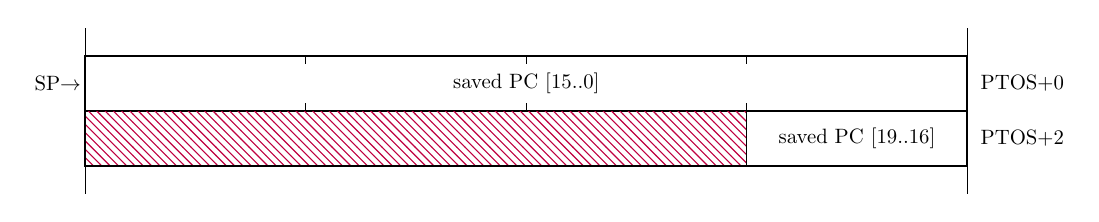
\begin{tikzpicture}[scale=0.7, every node/.style={scale=0.75}]
\draw[thick] (0,3) rectangle ++(16,1); \node at (8,3.5) {saved PC [15..0]};
\foreach \x in {4,8,12} { \draw (\x,3) -- ++(0,.15);  \draw (\x,4) -- ++(0,-.15); }
\draw[thick] (0,2) rectangle ++(16,1); \node at (14,2.5) {saved PC [19..16]};
%\draw[thick] (0,1) rectangle ++(16,1); \node at (8,1.5) {service identifier};
%\foreach \x in {4,8,12} { \draw (\x,1) -- ++(0,.15);  \draw (\x,2) -- ++(0,-.15); }
%\draw[thick] (0,0) rectangle ++(16,1); \node at (14,.5) {saved r11 [19..16]};
%\draw (12,0) -- ++(0,1);
%\draw[pattern=north west lines, pattern color=purple] (0,0) rectangle ++(12,1);
\draw[pattern=north west lines, pattern color=purple] (0,2) rectangle ++(12,1);
\foreach \x in {0,16} \draw (\x,1.5) -- (\x,4.5);
\node at (-.5,3.5) {SP$\rightarrow$};
\foreach \y/\offset in {3.5/0,2.5/2} \node at (17,\y) {PTOS+\offset};
\end{tikzpicture}
\label{fig:stacksc}
\end{figure}

When an interrupt is taken into account, the \lstinline{PC} and the \lstinline{SR} are pushed on the stack. To save space, the \lstinline{SR} is stored in the same 16-bit word as bits 19..16 of \lstinline{PC}. For an obscure reason, words are in reverse order and bits 19..16 of \lstinline{PC} are in high bits. The stack is shown at figure \ref{fig:stackit}.

\begin{figure}[h]
\caption{Stack in an interrupt handler}
\centering
\vspace{1em}
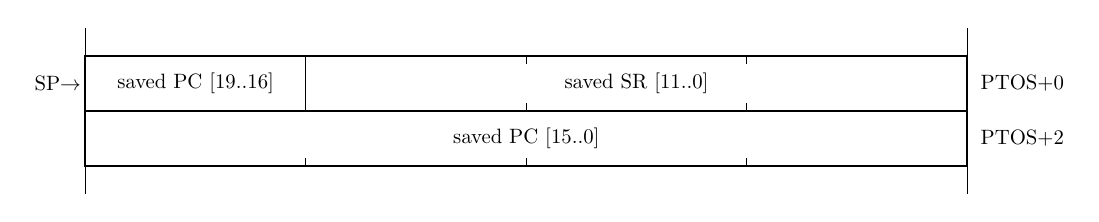
\begin{tikzpicture}[scale=0.7, every node/.style={scale=0.75}]
\draw[thick] (0,2) rectangle ++(16,1); \node at (8,2.5) {saved PC [15..0]};
\foreach \x in {4,8,12} { \draw (\x,2) -- ++(0,.15);  \draw (\x,4) -- ++(0,-.15); }
\draw[thick] (0,3) rectangle ++(16,1); \node at (2,3.5) {saved PC [19..16]}; \node at (10,3.5) {saved SR [11..0]};
\foreach \x in {4,8,12} { \draw (\x,3) -- ++(0,.15);  \draw (\x,4) -- ++(0,-.15); }
%\draw[thick] (0,1) rectangle ++(16,1); \node at (8,1.5) {saved r11 [15..0]};
%\foreach \x in {4,8,12} { \draw (\x,1) -- ++(0,.15);  \draw (\x,2) -- ++(0,-.15); }
%\draw[thick] (0,0) rectangle ++(16,1); \node at (14,.5) {saved r11 [19..16]};
\draw (4,3) -- ++(0,1);
%\draw[pattern=north west lines, pattern color=purple] (0,0) rectangle ++(12,1);
%\draw[pattern=north west lines, pattern color=purple] (0,2) rectangle ++(12,1);
\foreach \x in {0,16} \draw (\x,1.5) -- (\x,4.5);
\node at (-.5,3.5) {SP$\rightarrow$};
\foreach \y/\offset in {3.5/0,2.5/2} \node at (17,\y) {PTOS+\offset};
\end{tikzpicture}
\label{fig:stackit}
\end{figure}

\subsection*{Preemption cases}

A preemption can be synchronous or asynchronous. A synchronous preemption (SP) happens when a service call is done, for instance when a task activates a higher priority task. An asynchronous preemption (AP) happens under interrupt, for instance when a higher priority task is activated by an alarm. A preempted task may resume its execution following a synchronous event (SR) : the running task calls \lstinline{TerminateTask}, \lstinline{ChainTask}, \lstinline{WaitEvent} or \lstinline{SetEvent} or following an asynchronous event (AR) : an alarm does a \lstinline{SetEvent}. So there are 4 cases:.

\begin{description}

\item[SPSR] Synchronous Preemption, Synchronous Resume. $\tau_1$ is running, $\tau_2$ is ready. $P(\tau_1) > P(\tau_2)$.
$\tau_1$ calls \lstinline{WaitEvent} and is preempted synchronously, $\tau_2$ becomes running and  calls \lstinline{SetEvent}. $\tau_2$ is preempted and $\tau_1$ is resumed synchronously.

\item[SPAR] Synchronous Preemption, Asynchronous Resume. $\tau_1$ calls \lstinline{WaitEvent} ans is synchronously preempted, An alarm does a \lstinline{SetEvent} on $\tau_1$ which is asynchronously resumed.

\item[APSR] Asynchronous Preemption, Synchronous Resume. $\tau_1$ is running, $\tau_2$ is suspended. $P(\tau_1) < P(\tau_2)$. An alarm activates $\tau_2$, $\tau_1$ is asynchronously preempted, $\tau_2$ calls \lstinline{TerminateTask}, $\tau_1$ is synchronously resumed.

\item[APAR] Asynchronous Preemption, Asynchronous Resume. $\tau_1$ is running, $\tau_2$ is suspended. $P(\tau_1) < P(\tau_2)$. An alarm activates $\tau_2$, $\tau_1$ is asynchronously preempted. $\tau_2$ is terminated by the OS because of protection fault, for instance a timing protection interrupt and $\tau_1$ is asynchronously resumed.

\end{description}

So \emph{the stack frame has to be normalized}. The normalized stack frame is the asynchronous one shown at figure \ref{fig:stackit} because it contains the Status Register. Normalization is done at the beginning of the \sch. The end of the \sch is done using the \texttt{reti} instruction, as at the end of an interrupt.

The normalized stack frame may be done only when a context is saved to prevent a normalization if there is no context switch. However, the load of the context is much complicated, as the restauration of \texttt{r2} (aka status register) in the \sch re-enable the interrupts before the end of the function.

\section{The tpl\_sc\_handler}

The background color of the code snippets depends on the current active stack:
\begin{description}
	\item[green] process stack
	\item[red]   kernel stack
	\item[yellow] either kernel or process stack
\end{description}

%\fbox{\parbox{.99\textwidth}{The stack structure should be reviewed for the \lstinline{tpl_sc_handler}. Since volatile registers must be stacked first by an ISR, they should be at the bottom of the stack, just above the PC, and not at the top.}}

\vspace{1em}

The first thing to do is to compare the service id to the number of services to verify its validity.

\begin{lstlisting}[backgroundcolor=\color{yellow!15}]
    cmp #SYSCALL_COUNT, REG_SID
    jhs tpl_sc_handler_invalid_service_id
\end{lstlisting}

We need to have the same stack pattern for both the \sch\ and an interrupt handler which calls the operation system. Obviously volatile registers (r12 to r15 because we take into account both ABIs) are not saved in \sch\ since the caller does not expect their values to be preserved but we need to make room (8 bytes) on the stack for them because an interrupt handler will save these registers at this location. The 16 bit words at the bottom of this area is for the \lstinline{REG_RETARG} which is not saved yet.

\begin{lstlisting}[backgroundcolor=\color{yellow!15}]
    sub     #8, r1
\end{lstlisting}

The \sch\ needs one working register and we choose to use \lstinline{r11} which has to be saved on the process stack before using it.

\begin{lstlisting}[backgroundcolor=\color{yellow!15}]
    pushx.w r11
\end{lstlisting}

Then interrupts are disabled.

\begin{lstlisting}[backgroundcolor=\color{yellow!15}]
    dint
\end{lstlisting}

At that stage the stack is as follow:

\begin{center}
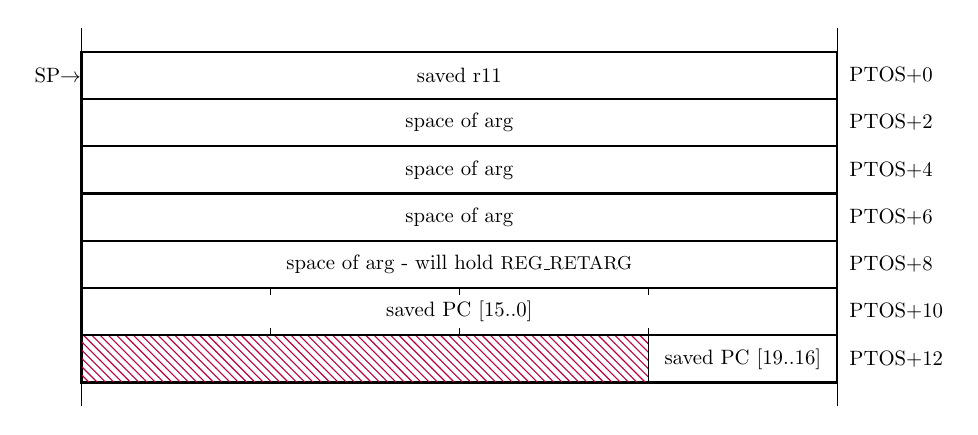
\begin{tikzpicture}[xscale=0.6, yscale=-.6, every node/.style={scale=0.75}]
\draw[thick] (0,0) rectangle ++(16,1); \node at (8,0.5) {saved r11};
\draw[thick] (0,5) rectangle ++(16,1); \node at (8,5.5) {saved PC [15..0]};
%\foreach \x in {4,8,12} { \draw (\x,6) -- ++(0,.15);  \draw (\x,7) -- ++(0,-.15); }
\draw[thick] (0,6) rectangle ++(16,1); \node at (14,6.5) {saved PC [19..16]};% \node at (10,5.5) {saved SR [11..0]};
\draw[pattern=north west lines, pattern color=purple] (0,6) rectangle ++(12,1);
\foreach \x in {4,8,12} { \draw (\x,5) -- ++(0,.15);  \draw (\x,6) -- ++(0,-.15); }
\draw (12,6) -- ++(0,1);
\foreach \y in {1,2,3} {
\draw[thick] (0,\y) rectangle ++(16,1); \node at ($(8,\y+.5)$) {space of arg};
}
\draw[thick] (0,4) rectangle ++(16,1); \node at ($(8,4.5)$) {space of arg - will hold {\small REG\_RETARG}};
\foreach \x in {0,16} \draw (\x,-.5) -- (\x,7.5);
\node at (-.5,0.5) {SP$\rightarrow$};
\foreach \offset in {0,2,...,12} \node[anchor=west] at ($(16.1,.5+.5*\offset)$) {PTOS+\offset};
\end{tikzpicture}
\end{center}



The bottom of the stack have to be updated to the normalized stack (i.e. the stack in an interrupt handler, figure \ref{fig:stackit}).

\begin{lstlisting}[backgroundcolor=\color{yellow!15}]
    mov     12(r1), r11    /* Saved PC [19..16] -> r11                  */
    mov     10(r1), 12(r1) /* Copy saved PC [15..0] at the good place   */
    swpb    r11            /* Get saved PC [19..16] in bits 11..8       */
    rlam.w  #4, r11        /* Shift them to bits 19..16                 */
    bis     r2, r11        /* Add the SR in its location at 11..0       */
    bis     #8, r11        /* set GIE bit (reset just before with dint) */
    mov     r11, 12(r1)    /* The stack is ok                           */
\end{lstlisting}

The stack is then as follow:

\begin{center}
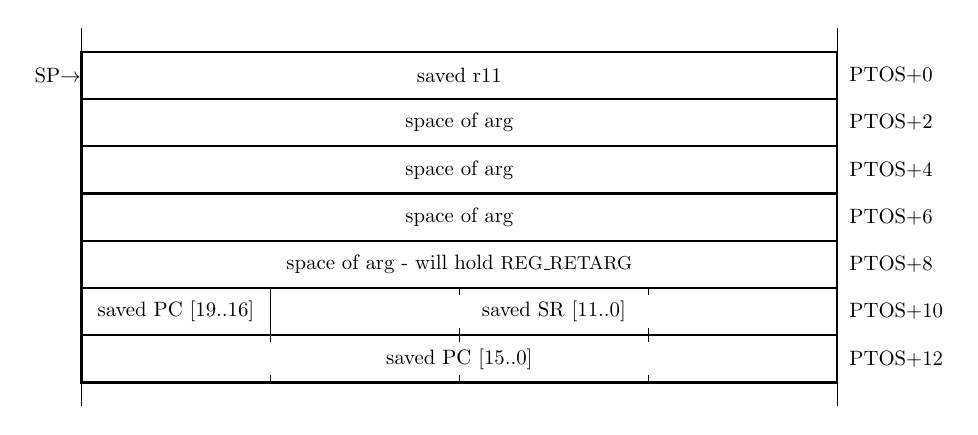
\begin{tikzpicture}[xscale=0.6, yscale=-.6, every node/.style={scale=0.75}]
\draw[thick] (0,0) rectangle ++(16,1); \node at (8,0.5) {saved r11};
\draw[thick] (0,6) rectangle ++(16,1); \node at (8,6.5) {saved PC [15..0]};
\foreach \x in {4,8,12} { \draw (\x,6) -- ++(0,.15);  \draw (\x,7) -- ++(0,-.15); }
\draw[thick] (0,5) rectangle ++(16,1); \node at (2,5.5) {saved PC [19..16]}; \node at (10,5.5) {saved SR [11..0]};
\foreach \x in {8,12} { \draw (\x,5) -- ++(0,.15);  \draw (\x,6) -- ++(0,-.15); }
\draw (4,5) -- ++(0,1);
\foreach \y in {1,2,3} {
\draw[thick] (0,\y) rectangle ++(16,1); \node at ($(8,\y+.5)$) {space of arg};
}
\draw[thick] (0,4) rectangle ++(16,1); \node at ($(8,4.5)$) {space of arg - will hold {\small REG\_RETARG}};
\foreach \x in {0,16} \draw (\x,-.5) -- (\x,7.5);
\node at (-.5,0.5) {SP$\rightarrow$};
\foreach \offset in {0,2,...,12} \node[anchor=west] at ($(16.1,.5+.5*\offset)$) {PTOS+\offset};
\end{tikzpicture}
\end{center}


The reentrancy counter is checked to prevent a switch to the kernel stack when executing a service called by a hook.

\begin{lstlisting}[backgroundcolor=\color{yellow!15}]
    tst.b &tpl_reentrancy_counter
    jnz   tpl_sc_handler_no_stack_switch
\end{lstlisting}

In case of stack switch, the process stack pointer (PSP) is saved on the kernel stack

\begin{lstlisting}[backgroundcolor=\color{red!15}]
    mov  r1,r11
    mov  #tpl_kern_stack_bottom, r1
    push r11
\end{lstlisting}

The kernel stack is as follow (\texttt{KTOS} stands for \emph{Kernel Top Of Stack}):

\begin{center}
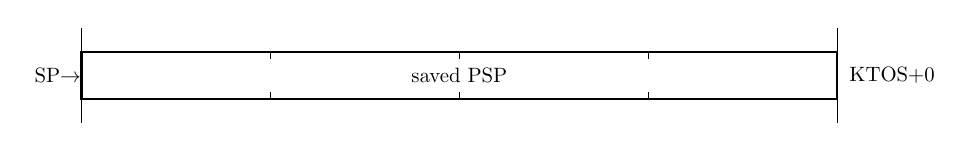
\begin{tikzpicture}[scale=0.6, every node/.style={scale=0.75}]
\draw[thick] (0,3) rectangle ++(16,1); \node at (8,3.5) {saved PSP};
\foreach \x in {4,8,12} { \draw (\x,3) -- ++(0,.15);  \draw (\x,4) -- ++(0,-.15); }
\foreach \x in {0,16} \draw (\x,2.5) -- (\x,4.5);
\node at (-.5,3.5) {SP$\rightarrow$};
\foreach \y/\offset in {3.5/0} \node[anchor=west] at (16.1,\y) {KTOS+\offset};
\end{tikzpicture}
\end{center}

Increment the reentrancy counter.

\begin{lstlisting}[backgroundcolor=\color{red!15}]
tpl_sc_handler_no_stack_switch:
    inc.b &tpl_reentrancy_counter
\end{lstlisting}

Init the \lstinline{NEED_SWITCH}/\lstinline{SAVE} in \lstinline{tpl_kern}.

\begin{lstlisting}[backgroundcolor=\color{red!15}]
    mov #tpl_kern, r11
    mov.b #NO_NEED_SWITCH_NOR_SCHEDULE, TPL_KERN_OFFSET_NEED_SWITCH(r11)
    mov.b #NO_NEED_SWITCH_NOR_SCHEDULE, TPL_KERN_OFFSET_NEED_SCHEDULE(r11)
\end{lstlisting}

Call the service.

\begin{lstlisting}[backgroundcolor=\color{red!15}]
    rla  REG_SID /* index -> offset */
    call tpl_dispatch_table(REG_SID)
\end{lstlisting}

From there, \lstinline{REG_RETARG} holds the return value. It is put at its location in the process stack. Also \lstinline{r13} and \lstinline{r14} become usable whatever is the ABI.

\begin{lstlisting}[backgroundcolor=\color{red!15}]
    pop	    r13 //get back PSP => r13
    movx.w  REG_RETARG, 8(r13) //put in Process's stack
\end{lstlisting}

Check the context switch condition in \lstinline{tpl_kern}.
\begin{lstlisting}[backgroundcolor=\color{red!15}]
    mov     #tpl_kern, r11
    tst.b   TPL_KERN_OFFSET_NEED_SWITCH(r11)
    jz      tpl_sc_handler_no_context_switch
\end{lstlisting}

Prepare the call to \lstinline{tpl_run_elected} by setting \lstinline{REG_RETARG} to 0, aka no save.
\begin{lstlisting}[backgroundcolor=\color{red!15}]
    mov     #0, REG_RETARG
\end{lstlisting}

Test the \lstinline{NEED_SAVE} condition.

\begin{lstlisting}[backgroundcolor=\color{red!15}]
    bit.b   #NEED_SAVE, TPL_KERN_OFFSET_NEED_SWITCH(r11)
    jz      tpl_sc_handler_no_save_running_context
\end{lstlisting}
Save the context. The MSP430 have a ``push multiple words", but no ``move multiple word". So, we get back to process stack to benefit this instruction

\begin{lstlisting}[backgroundcolor=\color{red!15}]
    mov     r1, r14	/* get a copy of the KSP to restore it later */
\end{lstlisting}
\begin{lstlisting}[backgroundcolor=\color{yellow!15}]
    mov     r13, r1	/* change stack to process stack */	
    pushm.w #7, r10	/* Push r4 to r10 on process stack (save) */
\end{lstlisting}
\begin{lstlisting}[backgroundcolor=\color{red!15}]
    mov     r14, r1	/* get back to kernel stack */
\end{lstlisting}

The whole context is now saved on process stack and the kernel stack has been cleaned. The saved context structure is shown at figure \ref{fig:context}.

\begin{figure}[h!]
\caption{Context saved on stack}
\begin{center}
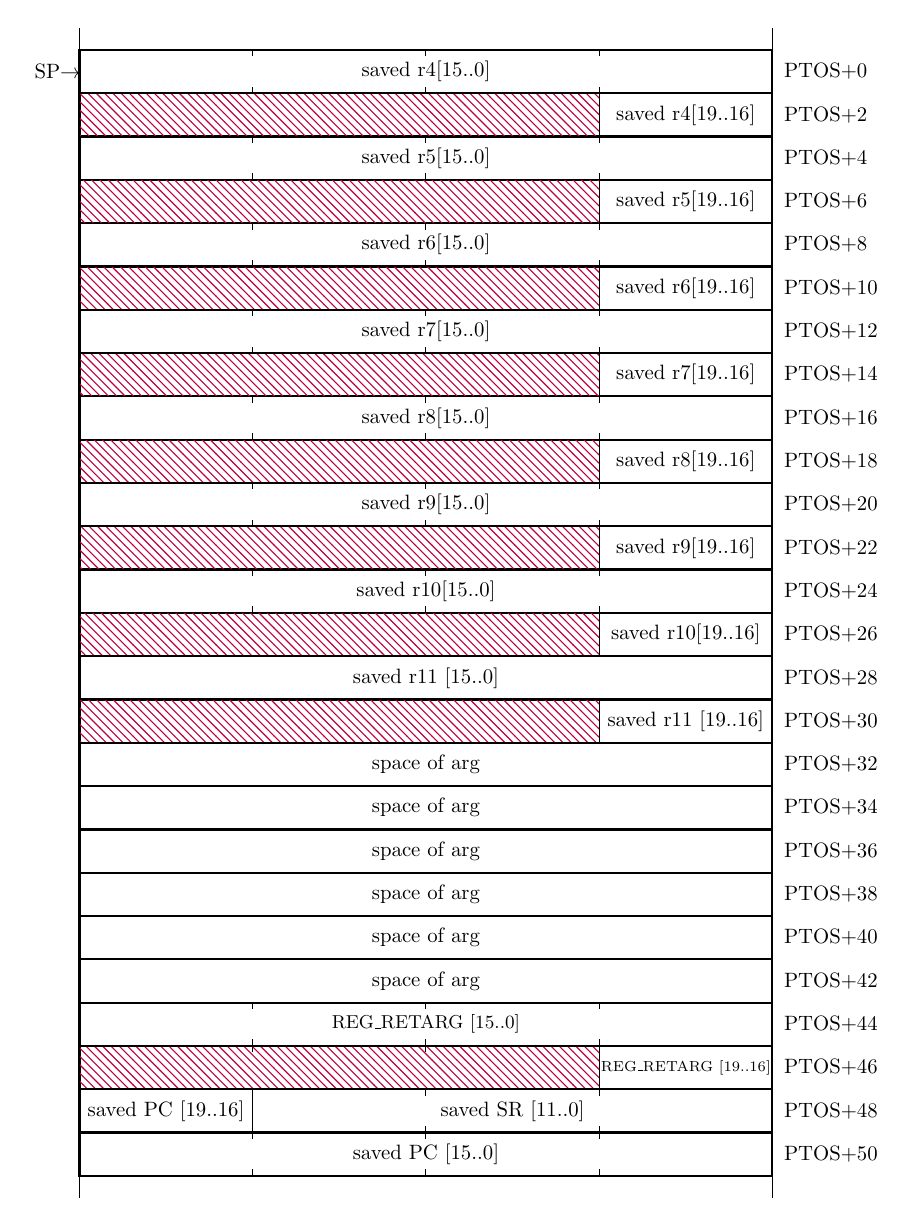
\begin{tikzpicture}[scale=0.55, every node/.style={scale=0.75}]

\foreach \reg/\y in {10/7,9/9,8/11,7/13,6/15,5/17,4/19} {
\draw[thick] ($(0,\y+8)$) rectangle ++(16,1); \node at ($(8,\y+8.5)$) {saved r\reg [15..0]};
\foreach \x in {4,8,12} { \draw ($(\x,\y+8)$) -- ++(0,.15);  \draw ($(\x,\y+9)$) -- ++(0,-.15); }
\draw[thick] ($(0,\y+7)$) rectangle ++(16,1); \node at ($(14,\y+7.5)$) {saved r\reg [19..16]};
\draw[pattern=north west lines, pattern color=purple] ($(0,\y+7)$) rectangle ++(12,1);
}

\draw[thick] (0,5) rectangle ++(16,1); \node at (8,5.5) {\small REG\_RETARG [15..0]};
\foreach \x in {4,8,12} { \draw (\x,23) -- ++(0,.15);  \draw (\x,5) -- ++(0,-.15); }
\draw[thick] (0,4) rectangle ++(16,1); \node at (14,4.5) {\scriptsize REG\_RETARG [19..16]};
\draw[pattern=north west lines, pattern color=purple] (0,4) rectangle ++(12,1);


\foreach \y in {6,7,...,11} {
\draw[thick] (0,\y) rectangle ++(16,1); \node at ($(8,\y+.5)$) {space of arg};
}

\draw[thick] (0,13) rectangle ++(16,1); \node at (8,13.5) {saved r11 [15..0]};
\foreach \x in {4,8,12} { \draw (\x,5) -- ++(0,.15);  \draw (\x,6) -- ++(0,-.15); }
\draw[thick] (0,12) rectangle ++(16,1); \node at (14,12.5) {saved r11 [19..16]};
\draw[pattern=north west lines, pattern color=purple] (0,12) rectangle ++(12,1);

\draw[thick] (0,2) rectangle ++(16,1); \node at (8,2.5) {saved PC [15..0]};
\foreach \x in {4,8,12} { \draw (\x,3) -- ++(0,.15);  \draw (\x,4) -- ++(0,-.15); }
\draw[thick] (0,3) rectangle ++(16,1); \node at (2,3.5) {saved PC [19..16]};
\draw[thick] (0,3) rectangle ++(16,1); \node at (10,3.5) {saved SR [11..0]};
\foreach \x in {4,8,12} { \draw (\x,2) -- ++(0,.15);  \draw (\x,3) -- ++(0,-.15); }
\draw (4,3) -- ++(0,1);
\foreach \x in {0,16} \draw (\x,1.5) -- (\x,28.5);
\node at (-.5,27.5) {SP$\rightarrow$};
\foreach \offset in {0,2,...,50} \node[anchor=west] at ($(16.1,27.5-.5*\offset)$) {PTOS+\offset};
\end{tikzpicture}
\end{center}
\label{fig:context}
\end{figure}

Now the stack pointer is saved in the dedicated location.

\begin{lstlisting}[backgroundcolor=\color{red!15}]
    mov     &tpl_kern, r11  /* Get the s_running slot of tpl_kern in r11 */
    mov     @r11, r11       /* Get the pointer to the context (SP alone) */
    mov     r13, @r11       /* Save the stack pointer                    */
\end{lstlisting}

Prepare the argument of \lstinline{tpl_run_elected} : 1 (aka save) and call it after switching back to the kernel stack.

\begin{lstlisting}[backgroundcolor=\color{red!15}]
    mov     #1, REG_RETARG
tpl_sc_handler_no_save_running_context:
    call    tpl_run_elected
\end{lstlisting}

\lstinline{tpl_run_elected} has copied the elected process slot of \lstinline{tpl_kern} to the \lstinline{running} slot. We load the stack pointer of the new running process.

\begin{lstlisting}[backgroundcolor=\color{red!15}]
    mov &tpl_kern, r11  /* Get the s_running slot of tpl_kern in r11 */
    mov @r11, r11       /* Get the pointer to the context (SP alone) */
\end{lstlisting}
\begin{lstlisting}[backgroundcolor=\color{yellow!15}]
    mov @r11, r1        /* Get the stack pointer                     */
\end{lstlisting}

Now, the context of the new running process is loaded. First we pop \lstinline{r4} to \lstinline{r10}

\begin{lstlisting}[backgroundcolor=\color{yellow!15}]
    popm.a #7,r10       /* Pop r4 to r10  */
	jmp tpl_sc_end_of_context_switch
\end{lstlisting}

The process stack is then as in figure \ref{fig:processStackLoaded}.

\begin{figure}[h!]
\caption{Process stack just loaded}
\begin{center}
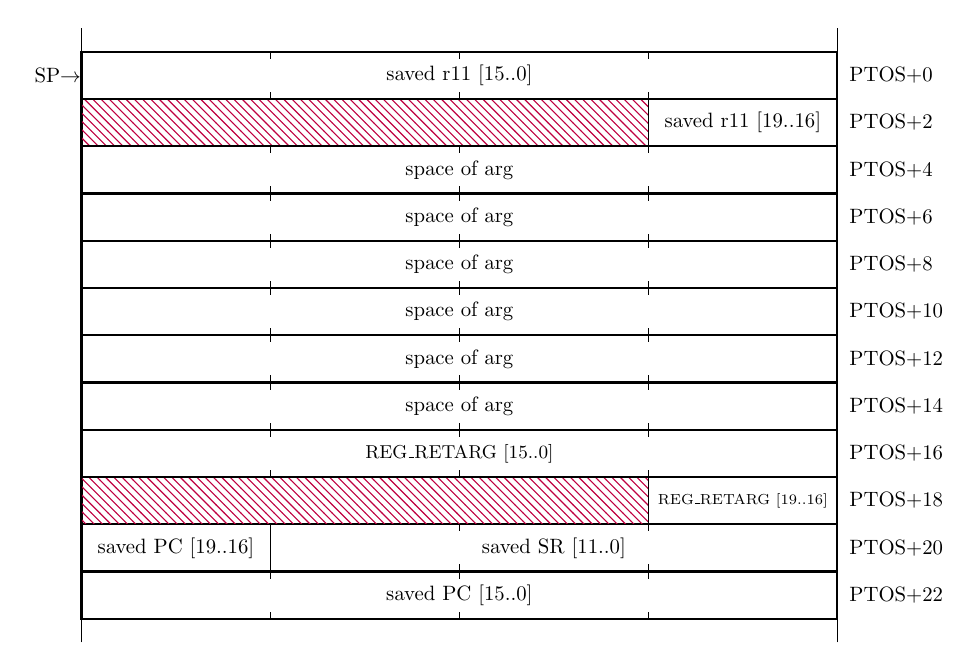
\begin{tikzpicture}[scale=0.6, every node/.style={scale=0.75}]
%\draw[thick] (0,7) rectangle ++(16,1); \node at (8,7.5) {saved r10 [15..0]};
%\foreach \x in {4,8,12} { \draw (\x,7) -- ++(0,.15);  \draw (\x,8) -- ++(0,-.15); }
%\draw[thick] (0,6) rectangle ++(16,1); \node at (14,6.5) {saved r10 [19..16]};
%\draw[pattern=north west lines, pattern color=purple] (0,6) rectangle ++(12,1);
\draw[thick] (0,13) rectangle ++(16,1); \node at (8,13.5) {saved r11 [15..0]};
\foreach \x in {4,8,12} { \draw (\x,13) -- ++(0,.15);  \draw (\x,14) -- ++(0,-.15); }
\draw[thick] (0,12) rectangle ++(16,1); \node at (14,12.5) {saved r11 [19..16]};
\draw[pattern=north west lines, pattern color=purple] (0,12) rectangle ++(12,1);
%\draw[thick] (0,3) rectangle ++(16,1); \node at (8,3.5) {saved PC [15..0]};
%\foreach \x in {4,8,12} { \draw (\x,3) -- ++(0,.15);  \draw (\x,4) -- ++(0,-.15); }
%\draw[thick] (0,2) rectangle ++(16,1); \node at (14,2.5) {saved PC [19..16]};
%\draw[pattern=north west lines, pattern color=purple] (0,2) rectangle ++(12,1);

\draw[thick] (0,2) rectangle ++(16,1); \node at (8,2.5) {saved PC [15..0]};
\foreach \x in {4,8,12} { \draw (\x,3) -- ++(0,.15);  \draw (\x,4) -- ++(0,-.15); }
\draw[thick] (0,3) rectangle ++(16,1); \node at (2,3.5) {saved PC [19..16]};
\draw[thick] (0,3) rectangle ++(16,1); \node at (10,3.5) {saved SR [11..0]};
\foreach \x in {4,8,12} { \draw (\x,2) -- ++(0,.15);  \draw (\x,3) -- ++(0,-.15); }
\draw (4,3) -- ++(0,1);


%\draw[thick] (0,1) rectangle ++(16,1); \node at (8,1.5) {service identifier};
%\foreach \x in {4,8,12} { \draw (\x,1) -- ++(0,.15);  \draw (\x,2) -- ++(0,-.15); }
%\draw[thick] (0,0) rectangle ++(16,1); \node at (14,.5) {saved r11 [19..16]};
%\draw (12,0) -- ++(0,1);
%\draw[pattern=north west lines, pattern color=purple] (0,0) rectangle ++(12,1);

\foreach \y in {6,7,...,11} {
\draw[thick] (0,\y) rectangle ++(16,1); \node at ($(8,\y+.5)$) {space of arg};
\foreach \x in {4,8,12} { \draw (\x,\y) -- ++(0,.15);  \draw ($(\x,\y+1)$) -- ++(0,-.15); }
}

\draw[thick] (0,5) rectangle ++(16,1); \node at ($(8,5.5)$) {\small REG\_RETARG [15..0]};
\foreach \x in {4,8,12} { \draw (\x,5) -- ++(0,.15);  \draw ($(\x,6)$) -- ++(0,-.15); }
\draw[thick] (0,4) rectangle ++(16,1); \node at ($(14,4.5)$) {\scriptsize REG\_RETARG [19..16]};
\draw[pattern=north west lines, pattern color=purple] (0,4) rectangle ++(12,1);

\foreach \x in {0,16} \draw (\x,1.5) -- (\x,14.5);
\node at (-.5,13.5) {SP$\rightarrow$};
\foreach \offset in {0,2,...,22} \node[anchor=west] at ($(16.1,13.5-.5*\offset)$) {PTOS+\offset};
\end{tikzpicture}
\end{center}
\label{fig:processStackLoaded}
\end{figure}

In case of no context switch, we have to get to the process stack, stored in r13

\begin{lstlisting}[backgroundcolor=\color{red!15}]
tpl_sc_handler_no_context_switch:
	mov r13, r1	 /* get back to process stack */
\end{lstlisting}
At last the reentrancy counter is decremented, r11 is restored, the \emph{space of args}, used in asynchronous preemption is removed from stack and the \lstinline{REG_RETARG} is poped.

Interrupts are enables during the \texttt{reti} instruction because it is related to the \texttt{GIE} bit in the status register.
\begin{lstlisting}[backgroundcolor=\color{yellow!15}]
tpl_sc_end_of_context_switch:
    dec.b  &tpl_reentrancy_counter
    jnz    tpl_sc_handler_still_in_kernel    

tpl_sc_handler_still_in_kernel:
    popx.a r11
    add    #12,r1       /* Skip volatile             */
    popx.a REG_RETARG   /* Get back the return value */
    reti
\end{lstlisting}

\subsection{Context initialisation}
The context that shoud be set during the task's initialisation (\texttt{tpl\_init\_context}) is the one of the figure \ref{fig:context}, but with a call to either \texttt{CallTerminateTask} or \texttt{CallTerminateISR2}, depending of the type of the process to init.

\emph{TODO} Works only with 16-bit register.Should be updated.

\begin{figure}[h!]
\caption{Context initialisation}
\begin{center}
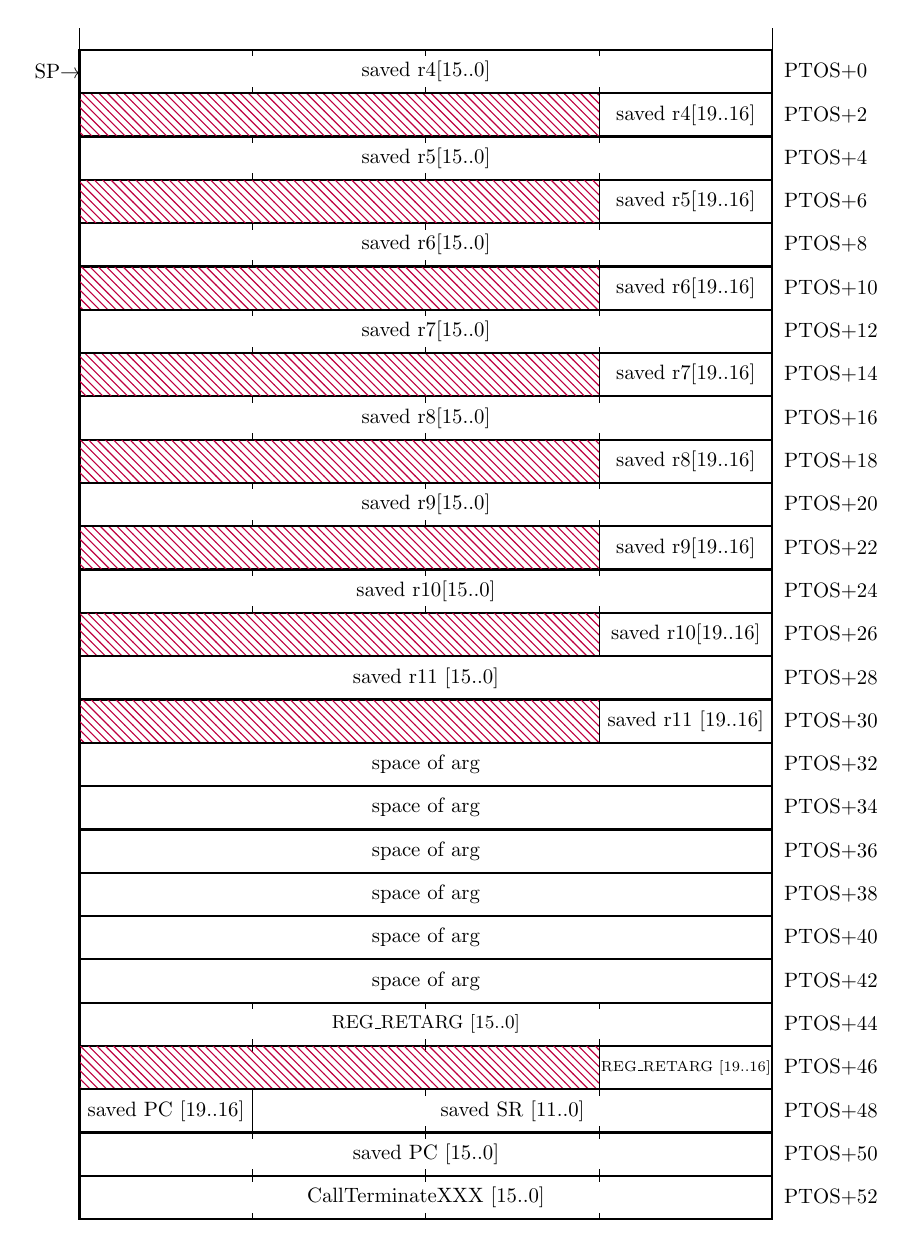
\begin{tikzpicture}[scale=0.55, every node/.style={scale=0.75}]

\foreach \reg/\y in {10/7,9/9,8/11,7/13,6/15,5/17,4/19} {
\draw[thick] ($(0,\y+8)$) rectangle ++(16,1); \node at ($(8,\y+8.5)$) {saved r\reg [15..0]};
\foreach \x in {4,8,12} { \draw ($(\x,\y+8)$) -- ++(0,.15);  \draw ($(\x,\y+9)$) -- ++(0,-.15); }
\draw[thick] ($(0,\y+7)$) rectangle ++(16,1); \node at ($(14,\y+7.5)$) {saved r\reg [19..16]};
\draw[pattern=north west lines, pattern color=purple] ($(0,\y+7)$) rectangle ++(12,1);
}

\draw[thick] (0,5) rectangle ++(16,1); \node at (8,5.5) {\small REG\_RETARG [15..0]};
\foreach \x in {4,8,12} { \draw (\x,23) -- ++(0,.15);  \draw (\x,5) -- ++(0,-.15); }
\draw[thick] (0,4) rectangle ++(16,1); \node at (14,4.5) {\scriptsize REG\_RETARG [19..16]};
\draw[pattern=north west lines, pattern color=purple] (0,4) rectangle ++(12,1);


\foreach \y in {6,7,...,11} {
\draw[thick] (0,\y) rectangle ++(16,1); \node at ($(8,\y+.5)$) {space of arg};
}

%\draw[thick] (0,6) rectangle ++(16,1); \node at (8,6.5) {saved r15};
%\foreach \x in {4,8,12} { \draw (\x,6) -- ++(0,.15);  \draw (\x,7) -- ++(0,-.15); }

\draw[thick] (0,13) rectangle ++(16,1); \node at (8,13.5) {saved r11 [15..0]};
\foreach \x in {4,8,12} { \draw (\x,5) -- ++(0,.15);  \draw (\x,6) -- ++(0,-.15); }
\draw[thick] (0,12) rectangle ++(16,1); \node at (14,12.5) {saved r11 [19..16]};
\draw[pattern=north west lines, pattern color=purple] (0,12) rectangle ++(12,1);

\draw[thick] (0,2) rectangle ++(16,1); \node at (8,2.5) {saved PC [15..0]};
\foreach \x in {4,8,12} { \draw (\x,3) -- ++(0,.15);  \draw (\x,4) -- ++(0,-.15); }
\draw[thick] (0,3) rectangle ++(16,1); \node at (2,3.5) {saved PC [19..16]};
\draw[thick] (0,3) rectangle ++(16,1); \node at (10,3.5) {saved SR [11..0]};
\foreach \x in {4,8,12} { \draw (\x,2) -- ++(0,.15);  \draw (\x,3) -- ++(0,-.15); }
\draw (4,3) -- ++(0,1);
\foreach \x in {0,16} \draw (\x,1.5) -- (\x,28.5);
\node at (-.5,27.5) {SP$\rightarrow$};
\foreach \offset in {0,2,...,52} \node[anchor=west] at ($(16.1,27.5-.5*\offset)$) {PTOS+\offset};
%22.5/0,21.5/2,20.5/4,19.5/6,18.5/8,17.5/10,16.5/12,15.5/14,14.5/16,13.5/18,
%12.5/20,11.5/22,10.5/24,9.5/26,8.5/28,7.5/30,6.5/32,5.5/34,4.5/36,3.5/38,2.5/40,
%1.5/42,0.5/44,-.5/46,-1.5/48,-2.5/50,-3.5/52,-4.5/54
%} \node[anchor=west] at ($(16.1,\y+7)$) {PTOS+\offset};
\draw[thick] (0,1) rectangle ++(16,1); \node at (8,1.5) {CallTerminateXXX [15..0]};
\foreach \x in {4,8,12} { \draw (\x,1) -- ++(0,.15);  \draw (\x,2) -- ++(0,-.15); }
\end{tikzpicture}
\end{center}
\label{fig:context}
\end{figure}


\section{The Systick Handler}

The Systick is generated by using a \lstinline{TIMERA} register. On the MSP430FR5969, \lstinline{TIMERA3} has been chosen. When entering the ISR, the stack is as shown at figure \ref{fig:stackit} and \lstinline{PC} (\lstinline{r0}) and \lstinline{SR} (\lstinline{r2}) have been saved. Before doing anything we have to save the volatile registers, which are \lstinline{r11}\footnote{r11 is not volatile in the \emph{MSPGCC} ABI but is volatile in \emph{GCC compiler for MSP} ABI. Anyway, in order to limit variabilility, \lstinline{r11} is saved for both ABIs.} to \lstinline{r15}, because they will not be saved when we will call the \lstinline{tpl_counter_tick_SystemCounter} C function.

\begin{lstlisting}[basicstyle=\footnotesize\ttfamily]
tpl_systick_handler:
    pushx.a REG_RETARG
#ifdef MSPGCC_ABI
    /* r15 has been pushed by pushx.a REG_RETARG */
    pushm.a #4, r14  /* Push r11, r12, r13, r14 */
#endif
#ifdef GCCFORMSP_ABI
    /* r12 has been pushed by pushx.a REG_RETARG */
    pushm.a #3, r15  /* Push r13, r14, r15 */
    pushx.a r11
#endif
\end{lstlisting}

As a result the stack is as follow for \emph{MSPGCC} ABI:

\begin{center}
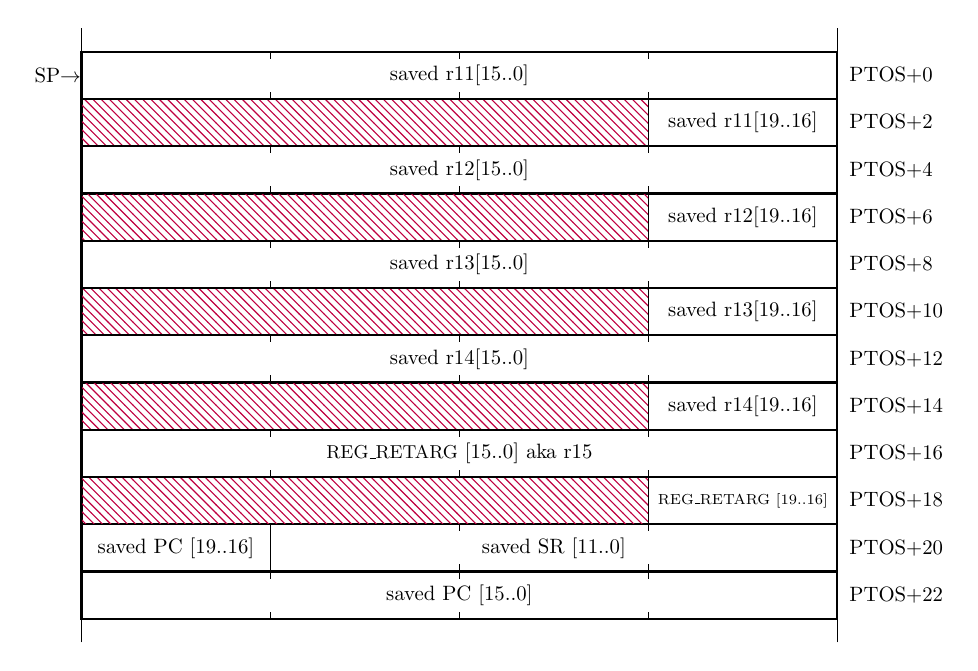
\begin{tikzpicture}[scale=0.6, every node/.style={scale=0.75}]
%\draw[thick] (0,7) rectangle ++(16,1); \node at (8,7.5) {saved r10 [15..0]};
%\foreach \x in {4,8,12} { \draw (\x,7) -- ++(0,.15);  \draw (\x,8) -- ++(0,-.15); }
%\draw[thick] (0,6) rectangle ++(16,1); \node at (14,6.5) {saved r10 [19..16]};
%\draw[pattern=north west lines, pattern color=purple] (0,6) rectangle ++(12,1);
%\draw[thick] (0,13) rectangle ++(16,1); \node at (8,13.5) {saved r11 [15..0]};
%\foreach \x in {4,8,12} { \draw (\x,13) -- ++(0,.15);  \draw (\x,14) -- ++(0,-.15); }
%\draw[thick] (0,12) rectangle ++(16,1); \node at (14,12.5) {saved r11 [19..16]};
%\draw[pattern=north west lines, pattern color=purple] (0,12) rectangle ++(12,1);
%\draw[thick] (0,3) rectangle ++(16,1); \node at (8,3.5) {saved PC [15..0]};
%\foreach \x in {4,8,12} { \draw (\x,3) -- ++(0,.15);  \draw (\x,4) -- ++(0,-.15); }
%\draw[thick] (0,2) rectangle ++(16,1); \node at (14,2.5) {saved PC [19..16]};
%\draw[pattern=north west lines, pattern color=purple] (0,2) rectangle ++(12,1);

\draw[thick] (0,2) rectangle ++(16,1); \node at (8,2.5) {saved PC [15..0]};
\foreach \x in {4,8,12} { \draw (\x,3) -- ++(0,.15);  \draw (\x,4) -- ++(0,-.15); }
\draw[thick] (0,3) rectangle ++(16,1); \node at (2,3.5) {saved PC [19..16]};
\draw[thick] (0,3) rectangle ++(16,1); \node at (10,3.5) {saved SR [11..0]};
\foreach \x in {4,8,12} { \draw (\x,2) -- ++(0,.15);  \draw (\x,3) -- ++(0,-.15); }
\draw (4,3) -- ++(0,1);


%\draw[thick] (0,1) rectangle ++(16,1); \node at (8,1.5) {service identifier};
%\foreach \x in {4,8,12} { \draw (\x,1) -- ++(0,.15);  \draw (\x,2) -- ++(0,-.15); }
%\draw[thick] (0,0) rectangle ++(16,1); \node at (14,.5) {saved r11 [19..16]};
%\draw (12,0) -- ++(0,1);
%\draw[pattern=north west lines, pattern color=purple] (0,0) rectangle ++(12,1);

%\foreach \y in {6,7,...,11} {
%\draw[thick] (0,\y) rectangle ++(16,1); \node at ($(8,\y+.5)$) {space of arg};
%\foreach \x in {4,8,12} { \draw (\x,\y) -- ++(0,.15);  \draw ($(\x,\y+1)$) -- ++(0,-.15); }
%}
\foreach \reg in {11,12,13,14} {
\draw[thick] ($(0,35-2*\reg)$) rectangle ++(16,1); \node at ($(8,35.5-2*\reg)$) {saved r\reg [15..0]};
\foreach \x in {4,8,12} { \draw ($(\x,35-2*\reg)$) -- ++(0,.15);  \draw ($(\x,36-2*\reg)$) -- ++(0,-.15); }
\draw[thick] ($(0,34-2*\reg)$) rectangle ++(16,1); \node at ($(14,34.5-2*\reg)$) {saved r\reg [19..16]};
\draw[pattern=north west lines, pattern color=purple] ($(0,34-2*\reg)$) rectangle ++(12,1);
}

\draw[thick] (0,5) rectangle ++(16,1); \node at ($(8,5.5)$) {{\small REG\_RETARG} [15..0] aka r15};
\foreach \x in {4,8,12} { \draw (\x,5) -- ++(0,.15);  \draw ($(\x,6)$) -- ++(0,-.15); }
\draw[thick] (0,4) rectangle ++(16,1); \node at ($(14,4.5)$) {\scriptsize REG\_RETARG [19..16]};
\draw[pattern=north west lines, pattern color=purple] (0,4) rectangle ++(12,1);

\foreach \x in {0,16} \draw (\x,1.5) -- (\x,14.5);
\node at (-.5,13.5) {SP$\rightarrow$};
\foreach \offset in {0,2,...,22} \node[anchor=west] at ($(16.1,13.5-.5*\offset)$) {PTOS+\offset};
\end{tikzpicture}
\end{center}
%\begin{center}
%\begin{tikzpicture}[scale=0.7, every node/.style={scale=0.75}]
%
%%\foreach \reg/\y in {15/} {
%%\draw[thick] (0,5) rectangle ++(16,1); \node at (8,5.5) {saved r11 [15..0]};
%%\foreach \x in {4,8,12} { \draw (\x,5) -- ++(0,.15);  \draw (\x,6) -- ++(0,-.15); }
%%\draw[thick] (0,4) rectangle ++(16,1); \node at (14,4.5) {saved r11 [19..16]};
%%\draw[pattern=north west lines, pattern color=purple] (0,4) rectangle ++(12,1);
%%}
%
%\draw[thick] (0,2) rectangle ++(16,1); \node at (8,2.5) {saved PC [15..0]};
%\foreach \x in {4,8,12} { \draw (\x,3) -- ++(0,.15);  \draw (\x,4) -- ++(0,-.15); }
%\draw[thick] (0,3) rectangle ++(16,1); \node at (2,3.5) {saved PC [19..16]};
%\draw[thick] (0,3) rectangle ++(16,1); \node at (10,3.5) {saved SR [11..0]};
%\foreach \x in {4,8,12} { \draw (\x,2) -- ++(0,.15);  \draw (\x,3) -- ++(0,-.15); }
%\draw (4,3) -- ++(0,1);
%\foreach \x in {0,16} \draw (\x,1.5) -- (\x,6.5);
%\node at (-.5,5.5) {SP$\rightarrow$};
%\foreach \y/\offset in {5.5/0,4.5/2,3.5/4,2.5/6} \node at (17,\y) {PTOS+\offset};
%\end{tikzpicture}
%\end{center}

And as follow for the \emph{GCC compiler for MSP} ABI:

\begin{center}
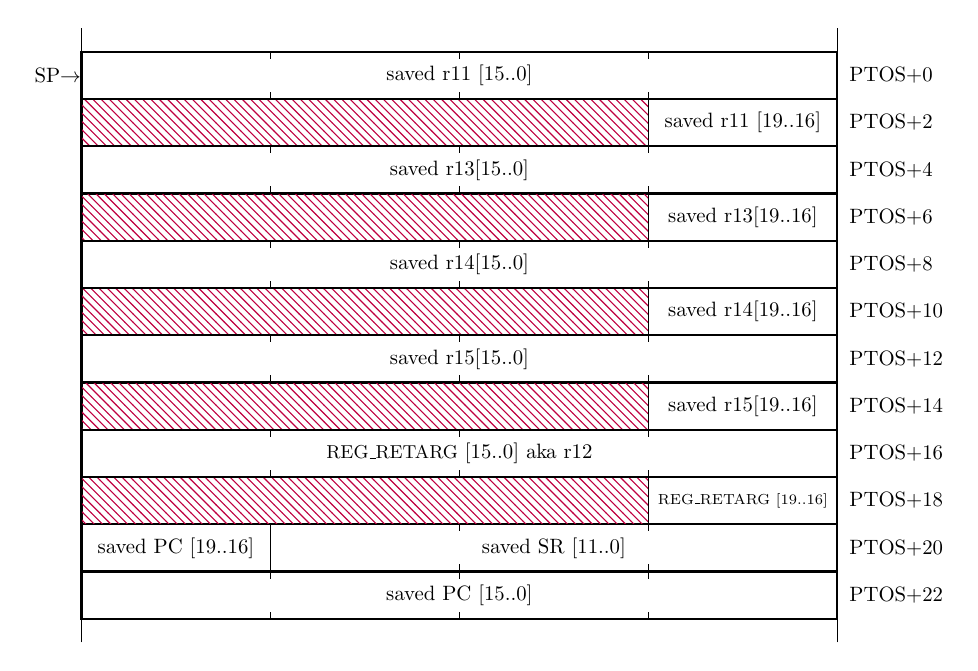
\begin{tikzpicture}[scale=0.6, every node/.style={scale=0.75}]
%\draw[thick] (0,7) rectangle ++(16,1); \node at (8,7.5) {saved r10 [15..0]};
%\foreach \x in {4,8,12} { \draw (\x,7) -- ++(0,.15);  \draw (\x,8) -- ++(0,-.15); }
%\draw[thick] (0,6) rectangle ++(16,1); \node at (14,6.5) {saved r10 [19..16]};
%\draw[pattern=north west lines, pattern color=purple] (0,6) rectangle ++(12,1);
\draw[thick] (0,13) rectangle ++(16,1); \node at (8,13.5) {saved r11 [15..0]};
\foreach \x in {4,8,12} { \draw (\x,13) -- ++(0,.15);  \draw (\x,14) -- ++(0,-.15); }
\draw[thick] (0,12) rectangle ++(16,1); \node at (14,12.5) {saved r11 [19..16]};
\draw[pattern=north west lines, pattern color=purple] (0,12) rectangle ++(12,1);
%\draw[thick] (0,3) rectangle ++(16,1); \node at (8,3.5) {saved PC [15..0]};
%\foreach \x in {4,8,12} { \draw (\x,3) -- ++(0,.15);  \draw (\x,4) -- ++(0,-.15); }
%\draw[thick] (0,2) rectangle ++(16,1); \node at (14,2.5) {saved PC [19..16]};
%\draw[pattern=north west lines, pattern color=purple] (0,2) rectangle ++(12,1);

\draw[thick] (0,2) rectangle ++(16,1); \node at (8,2.5) {saved PC [15..0]};
\foreach \x in {4,8,12} { \draw (\x,3) -- ++(0,.15);  \draw (\x,4) -- ++(0,-.15); }
\draw[thick] (0,3) rectangle ++(16,1); \node at (2,3.5) {saved PC [19..16]};
\draw[thick] (0,3) rectangle ++(16,1); \node at (10,3.5) {saved SR [11..0]};
\foreach \x in {4,8,12} { \draw (\x,2) -- ++(0,.15);  \draw (\x,3) -- ++(0,-.15); }
\draw (4,3) -- ++(0,1);


%\draw[thick] (0,1) rectangle ++(16,1); \node at (8,1.5) {service identifier};
%\foreach \x in {4,8,12} { \draw (\x,1) -- ++(0,.15);  \draw (\x,2) -- ++(0,-.15); }
%\draw[thick] (0,0) rectangle ++(16,1); \node at (14,.5) {saved r11 [19..16]};
%\draw (12,0) -- ++(0,1);
%\draw[pattern=north west lines, pattern color=purple] (0,0) rectangle ++(12,1);

%\foreach \y in {6,7,...,11} {
%\draw[thick] (0,\y) rectangle ++(16,1); \node at ($(8,\y+.5)$) {space of arg};
%\foreach \x in {4,8,12} { \draw (\x,\y) -- ++(0,.15);  \draw ($(\x,\y+1)$) -- ++(0,-.15); }
%}
\foreach \reg in {13,14,15} {
\draw[thick] ($(0,37-2*\reg)$) rectangle ++(16,1); \node at ($(8,37.5-2*\reg)$) {saved r\reg [15..0]};
\foreach \x in {4,8,12} { \draw ($(\x,37-2*\reg)$) -- ++(0,.15);  \draw ($(\x,38-2*\reg)$) -- ++(0,-.15); }
\draw[thick] ($(0,36-2*\reg)$) rectangle ++(16,1); \node at ($(14,36.5-2*\reg)$) {saved r\reg [19..16]};
\draw[pattern=north west lines, pattern color=purple] ($(0,36-2*\reg)$) rectangle ++(12,1);
}

\draw[thick] (0,5) rectangle ++(16,1); \node at ($(8,5.5)$) {{\small REG\_RETARG} [15..0] aka r12};
\foreach \x in {4,8,12} { \draw (\x,5) -- ++(0,.15);  \draw ($(\x,6)$) -- ++(0,-.15); }
\draw[thick] (0,4) rectangle ++(16,1); \node at ($(14,4.5)$) {\scriptsize REG\_RETARG [19..16]};
\draw[pattern=north west lines, pattern color=purple] (0,4) rectangle ++(12,1);

\foreach \x in {0,16} \draw (\x,1.5) -- (\x,14.5);
\node at (-.5,13.5) {SP$\rightarrow$};
\foreach \offset in {0,2,...,22} \node[anchor=west] at ($(16.1,13.5-.5*\offset)$) {PTOS+\offset};
\end{tikzpicture}
\end{center}

Switch to the kernel stack.

\begin{lstlisting}[basicstyle=\footnotesize\ttfamily]
    mov r1,r11                     /* Copy the PSP in r11        */
    mov #tpl_kern_stack_bottom, r1 /* Switch to the kernel stack */
    push r11                       /* Save PCP to kernel stack   */
\end{lstlisting}

The kernel stack is as follow:

\begin{center}
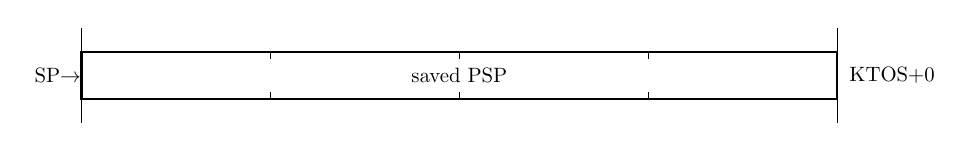
\begin{tikzpicture}[scale=0.6, every node/.style={scale=0.75}]
%\draw[thick] (0,7) rectangle ++(16,1); \node at (8,7.5) {saved r10 [15..0]};
%\foreach \x in {4,8,12} { \draw (\x,7) -- ++(0,.15);  \draw (\x,8) -- ++(0,-.15); }
%\draw[thick] (0,6) rectangle ++(16,1); \node at (14,6.5) {saved r10 [19..16]};
%\draw[pattern=north west lines, pattern color=purple] (0,6) rectangle ++(12,1);
%\draw[thick] (0,5) rectangle ++(16,1); \node at (8,5.5) {saved r11 [15..0]};
%\foreach \x in {4,8,12} { \draw (\x,5) -- ++(0,.15);  \draw (\x,6) -- ++(0,-.15); }
%\draw[thick] (0,4) rectangle ++(16,1); \node at (14,4.5) {saved r11 [19..16]};
%\draw[pattern=north west lines, pattern color=purple] (0,4) rectangle ++(12,1);
\draw[thick] (0,3) rectangle ++(16,1); \node at (8,3.5) {saved PSP};
\foreach \x in {4,8,12} { \draw (\x,3) -- ++(0,.15);  \draw (\x,4) -- ++(0,-.15); }
%\draw[thick] (0,2) rectangle ++(16,1); \node at (14,2.5) {saved PC [19..16]};
%\draw[pattern=north west lines, pattern color=purple] (0,2) rectangle ++(12,1);
%\draw[thick] (0,1) rectangle ++(16,1); \node at (8,1.5) {service identifier};
%\foreach \x in {4,8,12} { \draw (\x,1) -- ++(0,.15);  \draw (\x,2) -- ++(0,-.15); }
%\draw[thick] (0,0) rectangle ++(16,1); \node at (14,.5) {saved r11 [19..16]};
%\draw (12,0) -- ++(0,1);
%\draw[pattern=north west lines, pattern color=purple] (0,0) rectangle ++(12,1);
\foreach \x in {0,16} \draw (\x,2.5) -- (\x,4.5);
\node at (-.5,3.5) {SP$\rightarrow$};
\foreach \y/\offset in {3.5/0} \node[anchor=west] at (16.1,\y) {KTOS+\offset};
\end{tikzpicture}
\end{center}

Init the \lstinline{NEED_SWITCH}/\lstinline{SAVE} in \lstinline{tpl_kern}.

\begin{lstlisting}[basicstyle=\footnotesize\ttfamily]
    mov   #tpl_kern, r11
    mov.b #NO_NEED_SWITCH_NOR_SCHEDULE, TPL_KERN_OFFSET_NEED_SWITCH(r11)
    mov.b #NO_NEED_SWITCH_NOR_SCHEDULE, TPL_KERN_OFFSET_NEED_SCHEDULE(r11)
\end{lstlisting}

Call the function that increments the SystemCounter and manages alarm.

\begin{lstlisting}[basicstyle=\footnotesize\ttfamily]
    call tpl_counter_tick_SystemCounter
\end{lstlisting}

Switch back to the process stack

\begin{lstlisting}[basicstyle=\footnotesize\ttfamily]
    mov r1, r13 /* get a copy of the KSP to restore it later */
    pop r1      /* get the saved process stack pointer back  */
\end{lstlisting}

Check the context switch condition in \lstinline{tpl_kern}.

\begin{lstlisting}[basicstyle=\footnotesize\ttfamily]
    mov   #tpl_kern, r11
    tst.b TPL_KERN_OFFSET_NEED_SWITCH(r11)
    jz    tpl_systick_handler_no_context_switch
\end{lstlisting}

Save the rest of the context.

\begin{lstlisting}[basicstyle=\footnotesize\ttfamily]
    pushm.a #7, r10 /* Push r4 to r10 */
\end{lstlisting}

Now the stack pointer is saved in the dedicated location.

\begin{lstlisting}[basicstyle=\footnotesize\ttfamily]
    mov &tpl_kern, r11  /* Get the s_running slot of tpl_kern in r11 */
    mov @r11, r11       /* Get the pointer to the context (SP alone) */
    mov r1, @r11        /* Save the stack pointer                    */
\end{lstlisting}

Call \lstinline{tpl_run_elected} with argument 1 (aka save) after switching back to the kernel stack.

\begin{lstlisting}[basicstyle=\footnotesize\ttfamily]
    mov r13, r1         /* Switch back to the kernel stack         */
    mov #1, REG_RETARG
    add #2, r1          /* "pop" the PSP which is no longer useful */
    call tpl_run_elected
\end{lstlisting}

\lstinline{tpl_run_elected} has copied the elected process slot of \lstinline{tpl_kern} to the \lstinline{running} slot. We load the stack pointer of the new running process.

\begin{lstlisting}[basicstyle=\footnotesize\ttfamily]
    mov &tpl_kern, r11  /* Get the s_running slot of tpl_kern in r11 */
    mov @r11, r11       /* Get the pointer to the context (SP alone) */
    mov @r11, r1        /* Get the stack pointer                     */
\end{lstlisting}

Now, the context of the new running process is loaded. First we pop \lstinline{r4} to \lstinline{r10}

\begin{lstlisting}[basicstyle=\footnotesize\ttfamily]
    popm.a #7,r10       /* Pop r4 to r10  */
\end{lstlisting}



Restore the volatile registers and return from the interrupt handler.

\begin{lstlisting}[basicstyle=\footnotesize\ttfamily]
tpl_systick_handler_no_context_switch:

#ifdef MSPGCC_ABI
    /* r15 will be popped by popx.a REG_RETARG */
    popm.a #4, r14  /* Pop r11, r12, r13, r14 */
#endif
#ifdef GCCFORMSP_ABI
    /* r12 will be popped by popx.a REG_RETARG */
    popx.a r11
    popm.a #3, r15  /* Pop r13, r14, r15 */
#endif
    popx.a REG_RETARG
    reti
\end{lstlisting}

That's all !

\bibliographystyle{plain}
\bibliography{porting}

\end{document}  
